\documentclass{article}

\usepackage{natbib}
\usepackage{url}
\usepackage[a4paper, margin=3cm, lmargin=3.5cm]{geometry}

\title{Verification Notes}
\usepackage{setspace}
\usepackage{comment}
\usepackage{amsmath}
\usepackage{xcolor}

\linespread{1.3}

\begin{document}

\maketitle

\section{Paper Summaries}

\subsection{\citet{bom10}}
ACCESS uses the scheme of \citet{lock00} for mixing in unstable layers. 7 classification types for boundary layers. Cumulus mixing uses the mass-flux convection scheme. Entrainment rates across the inversion at the top of the boundary layer are parametrised using the eddy diffusivity scheme of Lock (1998; 2001) scaled using cloud-top cooling rates. Mixing in stable boundary layers uses the local Richardson number first order closure of \citet{louis79} with stability dependent surface exchanges calculated using Monin-Obukhov Similarity. 

\subsection{\citet{louis79}}

\subsection{\citet{lock00}}

\subsection{\citet{ecmwf18}}

\subsection{\citet{bishop13}}

\subsection{\citet{basu08}}

\subsection{\citet{kumar06}}

\subsection{\citet{zhang04}}
Great resource on character of diurnal cycle of winds in the PBL. Performs a comparison of five different parametrisation schemes. 

\subsection{\citet{holtslag13}}
Great summary article. Discusses evaluation studies of \citet{svensson11}. ``The modeled diurnal cycle of the 10-m wind speed does not resemble the observations in many cases, most models overestimate the wind speed during night, and the speed does not increase enough after the morning transition (Fig. 8b)." Also noted the importance of associating forecast scores with degree of mixing etc (page 1701). 

\subsection{\citet{hoxit75}}
Provides good figures showing the diurnal evolution of wind speed and direction. 

\subsection{\citet{englberger18}}
Discusses effect of PBL diurnal cycle on the wake structure of wind turbines and wind farms. 

\subsection{\citet{liu10}}
PBL height. 

\subsection{\citet{stensrud96}}
Low level jets. 

\subsection{\citet{svensson11}}
Evaluation of model performance. Crucial article. 

\subsection{\citet{zhang04}}
Quotes Dai and Deser paper reporting diurnal variability of surface winds could account for 50-70$\%$ of total wind variability. 

\subsection{\citet{mass02}}
Discusses predictability, and errors growing when horizontal resolution is reduced. Claims arguments of \citet{lorenz69} may be overly pessimistic. Notes that some studies have argued errors in synoptic forcing may contribute more to mesoscale errors than the mesoscale processes/resolutions themselves. Rotation suppresses energy cascade even at mesoscales, e.g. in supercells! ``It is clear that additional approaches should join the current verification toolbox. For example, one could verify the maximum wind or 1-h rainfall predicted by a forecast model over the subsequent day at a location. Time-averaged or spatially averaged parameters as well as model variability could be evaluated. Temporal or spatial shifting of model fields could be used to verify model structures. If suitable objective verification approaches can be devised, it may be possible to demonstrate increased value of high-resolution NWP."

\subsection{\citet{brooks93}}
Sounds warning about failure to implement ensemble forecasting, and the continuous drive toward higher resolution NWP. 

\subsection{\citet{lorenz69}}
Discusses different spatial and temporal scales of predictable motion.   

\subsection{\citet{lorenz82}}
Discusses upper and lower bounds of predictability in ECMWF.

\subsection{\citet{rife05}}
Comments on the need for ``feature based" mesoscale verification. This assumes that a forecast resolving a feature is better than one that doesn't even if the feature is spatiotemporally displaced. \citet{ebert00} provides one example of a feature based verification method. \textcolor{red}{But in my context, the ``features" being resolved by the higher resolution models, i.e. the additional random turbulence, are precisely what we're \textit{not} interested in!} \textcolor{blue}{It appears that the greatest benefit of the finer resolution is an increased ability to resolve the statistics of different scales of motion. In the present context this translates into improved forecasts of temporal variance, with the implication that the growth of errors is more realistic in the finer resolution \citep{rife05}.}

\subsection{\citet{pinson12}}
Proposes station-oriented view of the verification problem (which is what we are doing). Notes that there is a ``representativeness issue" in that station-data is resolving processes at physical scales the model is infact not intended to resolve. Notes that from the users perspective this is irrelevant. \textit{How could forecasters or post-processing incorporate this uncertainty into the forecast?} Discusses in detail the bilinear interpolation process for downscaling forecast data to location of stations. \textit{What is Jive's procedure for doing this?} Forecasts are benchmarked against 1-6 climatology based forecasts. Notes that observational uncertainty is known to be non-negligible, while surface effects introduce additional noise beyond what the numerical models intend to represent (or are capable of representing.) Representativeness issue ignored here for above reasons. Notes one method of dealing with observational uncertainty when performing ensemble (probabilistic) forecast verification is by transforming observations into random variables. Impact of observational uncertainty can then be assessed using methods like those of Pappenberger et al.~(2009). Note that Pappenberger still applies only to probabilistic forecasting. 

Very important - notes that the most poorly performing locations across Europe are the Alps and coastal regions, and that ``This could be expected since near-surface local effects [e.g. mountain and sea-breezes] are difficult to resolve at the fairly coarse resolution (50 km) of the ECMWF ensemble prediction system. [What is the spatial resolution of the ECMWF, ACCESS data used in GFE?] Authors comment on ``...questionable quality of the ensemble forecasts, for instance due to local effects not represented in a model with such a coarse spatial resolution". Could also be ensemble averaging process suppressing local processes.    

Key discussion - ``The periodic nature of the RMSE curves is linked to the diurnal cycles in the wind speed magnitude, the amplitude of such periodicities varying throughout Europe. To identify better the effect of the diurnal cycle on verification statistics, one may refine the analysis performed here by verifying forecasts depending on the time of the day (instead of the lead time), or by making a difference between forecasts issued at 0000 and 1200 UTC." So diurnal cycles are mentioned in passing here - good reference to make.  

Regarding observational uncertainty - the effect of uncertainty diminishes as the number of stations or the length of the evaluation period increases. ``This effect was observed to become negligible if looking at more than 100 stations over periods of more than a month (with two forecast series issued per day). For certain sites with strong local regimes though, one retrieves a more intuitive result that ensembles significantly underestimate wind speed.  

\subsection{\citet{lynch14}}
Focuses more on longer term forecasts. Interesting note that there is little difference in performance between 10m and 100m winds. Applies verification to forecast anomalies (from seasonal and diurnal cycles). SImilar approach to me, but work out average for each hour for each day of year, averaged over 32 years of ERA-Interim record. Note that I'm also avoiding the ``aritificial skill" associated with the seasonal cycle by restricting to just a particular season. I'm not convinced that seasonal skill is necessarily ``artificial" however! Both pinson and lynch use the CPRS score. Interesting notes on the large costs associated with wind farm station maintenance, and the need for probabilistic forecasts in order to manage these costs. 

\subsection{\citet{ebert08}}
Not easy to prove the value of mesoscale forecasts using traditional point-by-point verification results. At small scale features unpredictable - e.g. intermittant convective rainfall - in the example of winds the cold pool dynamics. Mesoscale forecasts typically verified against high-resolution gridded datasets, e.g. radar mosaics or reanalysis. Spatial verification techniques that do not require the forecasts to exactly match the observations at fine scales. Use of ``object oriented" techniques. The term `fuzzy' is consistent with the general concept of 'partial truth' introduced by Zadeh. Does Ebert's fuzzy scheme require gridded data? No. ``Fuzzy verification assumes that it is acceptable for the forecast to be slightly displaced and still be useful. Fuzzy concept can be applied in space or time. Really we're doing ``upscaling" rather than ``fuzzy" verification. Uncertainty in the observations represented by using neighbouring grid boxes. Less useful to me because ``event" framework not entirely appropriate to diurnal cycles. I am using an ``upscaling" approach. ``From the perspective of the forecast user, fuzzy verification gives important information on the scales and intensities at which the forecasts should be trusted."

\subsection{\citet{ebert00}}
N/A

\subsection{\citet{yates06}}
N/A

\subsection{\citet{mason08}}
Discusses practical methods for identifying in a yes/no sense whether a sea-breeze will occur. Discusses techniques for diagnosing speed and direction. Paper pretty old - would be good to have some references for up to date practices.  

\subsection{\citet{ferro17}}
Presents mathematical results regarding the calculation of verification statistics in the presence of observational error. 

\subsection{\citet{wilks11}}
Practical way to deal with autocorrelation is to think in terms of ``effective sample size" 
\begin{equation}
n' \approx n \frac{1-\rho_1}{1+\rho_1}.
\end{equation} 
Simply replace $n$ with $n'$ in appropriate places in $t$-test. 

\section{Notes}

\begin{enumerate}
\item
To investigate the impact these representation issues have on  discussed the WPI method outlined above is modified so that the performance of the Official forecast can    Two methods are used to investigate how the representation issues discussed above effect verification statistics of the diurnal wind cycle.   
\item
To assess how well the diurnal perturbations of an overall region are predicted, for instance those of the Victorian coastal station group (see Fig. \ref{Fig:station_map}), the perturbations across each station group are averaged before WPI values calculated. The temporal means and sampling distributions of the WPI are then calculated as before, with each value of WPI calculated from the spatially averaged perturbations treated as a single observation. This provides a conservative method for dealing with spatial correlation in the perturbations.        
\item
One factor that complicates interpretation of statistics of WPI, is that the near surface winds observed in AWS data are consistently noisier than those of the Official, ECMWF and ACCESS forecasts. This is likely due to unresolved subgrid scale turbulence in the Official, ECMWF and ACCESS model datasets. It would be unreasonable to expect forecasters to be able to predict this essentially random additional observed variability, and so a direct comparison of observed and modelled diurnal cycles is overly stringent. 
\item
Note that subtracting background winds may raise concerns, because perturbations obviously depend on background winds. However, the forecaster does not have knowledge of the observations when they make the diurnal process edits. They are implicitly assuming that the true mean state will be close enough to the predicted mean state - however this prediction is produced - to justify making diurnal edits on the basis of the predicted mean state.
\item
To reduce the significance of unpredictable noise, we also compare temporal averages of the perturbations for each dataset. These comparisons have less operational significance: people generally care how well the actual weather forecast performed, not whether the average of a predicted quantity matched the average of an observed quantity. However, comparisons of averages arguably better represent what we can realistically expect from human forecaster edits, and from weather forecasts overall, particularly in regards to small scale processes like sea-breezes. Furthermore, when temporal averages of perturbations are considered, the diurnal signal becomes dramatically clearer, and structual differences become much easier to diagnose. 
\item
To quantify how closely the temporally averaged Official forecast perturbations match those of the AWS observations, we calculate 
$\left\lvert \overline{\boldsymbol{u}}_{\text{AWS}} - \overline{\boldsymbol{u}}_{\text{O}} \right\rvert$ for each hour. To assess the performance of the Official temporally averaged perturbations against those ACCESS,
\item
Two edits are commonly involves changing the surface wind fields near coastlines to try to represent sea-breezes more realistically. Forecasters invest time in making sea-breeze edits because accurate predictions of near-surface winds are highly valued by a number of users, such as the aviation and energy \citep{smith09} industries. Accurate sea-breeze forecasts are also valuable to environmental monitoring authorities, as these winds provide ventilation to coastal urban areas.
\item
Assessing the accuracy of a weather forecast is a task far more nuanced than it might first appear. For instance, attempting to assess the accuracy of a precipitation forecast by comparing the rainfall amounts measured at an individual weather station to the closest grid point of a model prediction will often give poor results. Although the synoptic drivers of convection are usually well predicted, excatly where convective cells form, and where the most rain falls, is highly unpredictable. As such, it is often appropriate to use ``fuzzy" verification metrics which measure the agreement between prediction and observation in a more indirect way. For instance, one approach known as ``upscaling" is to first average forecast and observational data over a given spatial domain before calculating verification scores. \citet{ebert08} provided a review of current ``fuzzy verification" methodologies, and a framework for how they can be used to determine the spatial scales at which a given forecast has predictive skill.
\item
\citet{lynch14} also performed a verification study of ECMWF 10 m wind speed data, with the goal of assessing skill at lead times of between 14 to 20 days. They compared ECMWF 32-day forecast model wind speeds with gridded ERA-Interim wind speeds between 2008-12, with both datasets analysed at a six hour temporal resolution. Before conducting the comparison, the wind speed data were transformed into wind-speed ``anomaly" data by first calculating the mean wind speed at 0000, 0600, 1200 and 1800 UTC for each calendar day from the entire ERA-Interim record, and from a 20 year ECMWF 32-day model hindcast, then subtracting these means from the ERA-Interim and ECMWF 32-day model data respectively. Wind speed anomaly data was used so that stable seasonal and diurnal cycles did not contribute to verification scores. At the 14-20 day timescale around western Europe, the greatest skill was found in the boreal winter (austral summer) months of December, January and February.  
\item
\citet{pinson12} and \citet{lynch14} restricted their verification studies to wind speeds, but wind directions are also crucial to diagnosing whether land sea breezes - and the diurnal wind cycle more generally - are being forecast correctly. Furthermore, no previous published work has proposed a verification methodology to assess the accuracy of the diurnal wind cycle in forecasts, or of the contributions made to this accuracy by human forecaster edits of model output. Finally, no previously published work has considered the performance of ACCESS near surface winds, which together with ECMWF, are the model guidance products most widely used by Australian forecasters.
\item
Example figure with one day diurnal cycles for both AWS, Official, ECMWF and ACCESS winds, perturbations, and perturbation climatology. Just one season.
\item
Airport breakdown for one season, WPI, CWPI for one season, for both ACCESS and ECMWF. Second season in online supporting material.
\item
Example results for straight coastlines - perhaps north, northeast, northwest, south, southeast, southwest? Again, just do one season, include second season in online supporting material?
\item
Look at timing results by fitting ellipses and checking orientations of major axes. Just one season - both ECMWF and ACCESS? Maybe just ACCESS if ECMWF results are dodgy?
\item
Confirm ACCESS and ECMWF are indeed the msot commonly used model guidance products for winds. 
\item
I tried modifying the pressure perturbation terms $\frac{A}{\pi} + \frac{A}{2} \cos \left(\omega t\right)$ so that the new ellipse fit of equations (\ref{Eq:u}) and (\ref{Eq:v}) are now solutions to equations (\ref{Eq:h_u}) and (\ref{Eq:h_v}), but with no luck. For example, simply changing to $\frac{A}{\pi} + \frac{A}{2} \cos \left(\alpha\left(\psi,t\right)\right)$ doesn't work, nor does expanding this expression as a Fourier series and solving each term individually. This doesn't really matter anyway as my main argument is that this two-dimensional model cannot capture boundary layer mixing processes.
\end{enumerate}

\begin{enumerate}
\item
In Cairns and Townsville (austral summer), ECMWF understimates the magnitude of the land-sea breeze, leading to ACCESS resolving the diurnal cycle more accurately. During austral winter ECMWF again underperfoms, but (Townsville) more to do with shape of the hodograph and direction of the sea-breeze. At Cairns, it's essentially again because the ECMWF peak seabreeze is slightly (1 knot) too slow.   
\item
In Darwin - ACCESS perturbations bizarre during austral summer (wet season), but ECMWF also much too weak (about half the amplitude). 
\item
In Darwin - during austral winter (dry season) - ECMWF very accurate - gets peak of sea-breeze perfectly correct! Also resolves weird bump at 12 UTC quite well. However, does not resolve bump at 1 UTC at all. ACCESS doesn't either really. 
\item
Interesting - at Melbourne ECMWF and ACCESS essentially agree, but both underestimate the magnitude of the land-sea breeze. True of both seasons. 
\item
Adelaide - ACCESS and ECMWF almost match at Adelaide. Amplitudes generally slightly too weak compared to observations however. 
\item
Need to assume independence of measurement and rounding error in observations. 
\item
The two most important results of section \ref{Sec:Results} to explain are, first, why equations \ref{Eq:u} and \ref{Eq:v} provide such a good fit to the climatological perturbations and, second, why there are such substantial changes in the performance of the Official forecast at the different spatial and temporal scales. 

The idea of applying an ellipse fit to the diurnal cycle of surface winds originated with \citet{haurwitz47}, and was later extended by \citet{kusuda83}, who obtained exact solutions for $u$ and $v$ resembling equations (\ref{Eq:u_h}) and (\ref{Eq:v_h}) for the simple model
\begin{align}
\frac{du}{dt} - fv + ku &= F_x - F(t), \label{Eq:h_u}\\
\frac{dv}{dt} + fu + kv &= F_y, \label{Eq:h_v}
\end{align}
where $u$, $v$ are taken in a coordinate system where the $x$ axis is normal to the coast, $f$ is the Coriolis parameter, $k$ is a linear friction coefficient, $\left(F_x, F_y\right)$ represents a constant synoptic scale pressure gradient force, $\omega$ is the angular frequency of earth's rotation, and 
\begin{equation}
F(t) = \frac{A}{\pi} + \frac{A}{2} \cos \left(\omega t\right)
\end{equation}
is the pressure gradient force normal to the coastline induced by the diurnally varying air temperature contrast over the land and sea surfaces. The obvious limitations of this model are discussed extensively by \citet{haurwitz47} and \citet{kusuda83}, but the most important for our purposes involve the choice of $F(t)$, which does not sufficiently capture the asymmetries between daytime heating and nighttime cooling \citep[e.g.][]{svensson11}, and the fact that the model has no vertical dimension, and therefore cannot capture the boundary layer mixing processes that play a significant role in the diurnal wind cycle \citep[e.g.][]{hoxit75}. \textcolor{red}{Note that I tried modifying the pressure perturbation terms $\frac{A}{\pi} + \frac{A}{2} \cos \left(\omega t\right)$ so that the new ellipse fit of equations (\ref{Eq:u}) and (\ref{Eq:v}) become solutions to equations (\ref{Eq:h_u}) and (\ref{Eq:h_v}), but with no luck. For example, simply changing to $F(t)$ to $\frac{A}{\pi} + \frac{A}{2} \cos \left(\alpha\left(\psi,t\right)\right)$ doesn't work, nor does expanding this expression as a Fourier series and solving each term individually.} 

\citet{gille05} applied this fit to satellite scatterometer wind observations, which after temporal averaging provided only four temporal datapoints at each $0.25^\circ \times 0.25^\circ$ spatial grid cell. As such, their fit was very good, explaining over $90\%$ of the wind variability in each spatial gridcell. However, the choice of ellipse parametrisation in equations \ref{Eq:u} and \ref{Eq:v} assumes that datapoints lie on the ellipse at equal intervals of time $t$. When observational or model data with an hourly or smaller timestep is considered, this assumption becomes too stringent, as heating asymmetries imply that wind perturbations evolve much more rapidly during the day than at night (see Fig. XX). \textcolor{red}{Note I'm also basing this point on knowledge of the land vs sea breeze, and knowledge of heating vs cooling asymmetries \citep[][e.g.]{brown17}.} 
\end{enumerate}

\begin{comment}
The methods developed in this study can be readily extended to analyse \emph{just} the sea-breezes satisfying the operational definition above. For instance, to study the sea-breezes at a station near a coastline with inward pointing normal vector $\widehat{\boldsymbol{n}}$, the wind perturbation datasets could be restricted to just those days where the corresponding raw wind vector $\boldsymbol{u}$ satisfies $\widehat{\boldsymbol{n}} \cdot \boldsymbol{u} > 0$ for at least one of the hours of that day.

How much time should forecasters spend on sea-breeze edits (if any)? What is the value of an improved diurnal cycle climatology? Improving the accuracy of forecast climatologies will have little value to the typical forecast user. Are there applications where a higher performing climatological forecast yields better outcomes, even if errors increase or even get worse? 

Increasing the resolution of a forecast may reduce bias, but increase error.

Error, not bias, that generally matters for the forecast user. Standard methods for ``improving" forecasts (adding parametrisations, increasing resolution) reduce bias, but actually increase errors! 

Although they have similar definitions, $\overline{\text{WPI}}$ and CWPI measure different things. They do not converge as the length of the time period grows - they don't even necessarily approach the same sign. As a simple example, suppose that for each day, the observed and Official wind perturbations are given by $\boldsymbol{p}_{\text{AWS}} = \left(5\cos\omega t , 5\sin\omega t\right)$ and $\boldsymbol{p}_\text{O} = \left(6\cos\omega t , 6\sin\omega t\right)$, respectively. Furthermore, suppose that the ACCESS perturbations alternate between $\boldsymbol{p}_{\text{A}} = \left(7\cos\omega t , 7\sin\omega t\right)$ and $\boldsymbol{p}_{\text{A}} = \left(3\cos\omega t , 3\sin\omega t\right)$ from one day to the next. Then for any contiguous period of $n$ days, $\overline{\text{WPI}} = 2 - 1 = 1$, but $\text{CWPI} \approx -1$, with the approximation becoming exact for even $n$. Moreover $\overline{\text{WPI}}=1$ with a confidence of 1, and using the bootstrapping procesure described above, the confidence that $\text{CWPI} = -1$ approaches 1 as $n\to \infty$. This example shows that while the WPI and CWPI are sensitive both to random error and consistent biases between the different datasets, the CWPI becomes increasingly less sensitive to random error as the length of the time period being considered grows. Thus while the WPI arguably provides a more meaningful operational metric, as it measures the accuracy of actual forecast data, it may favour a more biased dataset over a less biased one, just because the internal variability of that dataset is lower. One consequence of this is that model data at a lower spatiotemporal resolution may outperform in $\overline{\text{WPI}}$ model data of a higher resolution, purely because the internal variability is lower. In this way, the CWPI may actually provide more information about the performance of different forecasts.

Note that the Bureau has not yet moved to ensemble forecasting - and probabilistic verification methods are therefore not appropriate. 
\end{comment}


the Adelaide Airport and Adelaide Airport station group results in Fig.~\ref{Fig:error_decomp_sa} can be explained by the fact that 

  Similar observations can be made for other locations considered in this study, with the exception of the NT station groups, where zonal biases in ECMWF at around 02:00 UTC at all three spatial scales explain why Official outperforms ECMWF around this time in the WPI results of Figs.~\ref{Fig:wpi_coastal} c) and d), and Fig.~\ref{Fig:airport_wpi}.           

perturbations are much greater than those of ECMWF, At the scale of the individual airport station, the variance of the AWS perturbations is much larger than any of the other datasets, but this difference in variability decreases at coarser spatial scales. At the airport station scale, the additional variability in AWS is mostly uncorrelated to Official or ECMWF, explaining the noisy results of Figs.~\ref{Fig:airport_wpi} a) and b). At the intermediate airport station group scale, the variances of



Applying equation (\ref{Eq:MSE}) to each dataset reveals that at all scales, the variances of the Official perturbations are much greater than those of ECMWF, At the scale of the individual airport station, the variance of the AWS perturbations is much larger than any of the other datasets, but this difference in variability decreases at coarser spatial scales. At the airport station scale, the additional variability in AWS is mostly uncorrelated to Official or ECMWF, explaining the noisy results of Figs.~\ref{Fig:airport_wpi} a) and b). At the intermediate airport station group scale, the variances of the AWS perturbations are of similar magnitude to those of Official, but larger than those of ECMWF, explaining ECMWFs almost complete outperformance of Official in Figs.~\ref{Fig:airport_wpi} c) and d)             

to each dataset reveals that ECMWF generally outperforms Official in the airport station group results of Figs.~\ref{Fig:airport_wpi} c) and d) 


Figure \ref{Fig:error_Official} shows each term in the mean square error (MSE) decomposition of equation (\ref{Eq:MSE}) for Darwin Airport, the Darwin Airport station group, and the NT coastal station group. These station groups provide interesting examples, as Fig.~\ref{Fig:airport_wpi} indicates that in this region at small scales the Official forecast produces lower absolute errors than ECMWF at around 02:00 UTC, in contrast to most other locations. At Darwin airport, the MSE is dominated by the variance terms, although the contribution of the variance terms to the MSE is reduced after averaging over either the Darwin Airport or NT coastal station groups, with the bias terms now dominant at certain times. Figure \ref{Fig:nt_ellipse_hodo} b) and c) shows that the biases in the zonal and meridional perturbations at the two larger scales reflect amplitude and direction biases in Official's temporal hodograph, likely resulting from forecaster edits that overly strengthen the sea-breeze. 

Figure \ref{Fig:error_ECMWF} provides the analogous MSE decompositions for ECMWF. The variance of the ECMWF perturbations is significantly lower than for Official, resulting in generally lower total variance terms. However, ECMWF features significant zonal biases between 20:00 and 04:00 UTC, which are also present in Official at the two coarser spatial scales. Note that the MSEs of Official and ECMWF are closely related to $\overline{\text{WPI}}_\text{OE}$, which is the difference between the mean absolute errors of Official and ECMWF; similarly, the squared bias components of the MSE are closely related to $\text{CWPI}_\text{OE}$. 

ECMWF's large zonal biases at 02:00 UTC explain why Official produces lower absolute errors than ECMWF, and hence positive $\overline{\text{WPI}}_\text{OE}$ values in Figs.~\ref{Fig:wpi:coastal} and \ref{Fig:airport_wpi} at this time. Official's large biases over the two coarser scales contribute to the negative $\overline{\text{WPI}}_\text{OE}$ values in Fig.~\ref{Fig:airport_wpi} between 06:00 and 10:00 UTC, although $\overline{\text{WPI}}_\text{OE}$ remains negative when both ECMWF and Official have low bias, such as at 14:00 UTC, because of Official's higher total variance term. This higher total variance occurs because the Official perturbations exhibit more variance than those of ECMWF, but are not always sufficiently correlated with the AWS perturbations. 

At Darwin Airport, $\mse\left(u_\text{AWS}, u_\text{O}\right)$ exceeds $\mse\left(u_\text{AWS}, u_\text{E}\right)$ from 04:00 to 16:00 UTC due to higher total variance, whereas outside of these times $\mse\left(u_\text{AWS}, u_\text{E}\right)$ exceeds $\mse\left(u_\text{AWS}, u_\text{O}\right)$ due to larger bias. The higher total variance of $u_\text{AWS} - u_\text{O}$ occurs because $\var\left(u_\text{O}\right) > \var\left(u_\text{E}\right)$. This additional variability is mostly random from 04:00 to 14:00 UTC, i.e. $u_\text{O}$ is not sufficiently correlated with $u_\text{AWS}$ at these times for the additional variability of $u_\text{O}$ to produce a reduction in mean square error. Thus, while the bias between Official and AWS is lower, or about the same, as that between ECMWF and AWS, the higher variability of Official results in higher mean square error for most of the day. Figure \ref{Fig:error_decomp_v} shows similar conclusions can be drawn for the meridional perturbations at Darwin Airport, although in this case $\var\left(u_\text{O}\right) > \var\left(u_\text{E}\right)$ for the entire day. Most of the difference between the WPI and CWPI scores for the Official versus ECMWF comparison at Darwin Airport in Figures \ref{Fig:airport_wpi} and \ref{Fig:airport_cwpi}, respectively, can be explained through the different mean square error and bias terms for the zonal perturbations alone. 



Figure \ref{Fig:nt_ellipse_hodo} a) shows that ECMWF's climatological perturbations at Darwin Airport underestimate the easterly perturbations from 00:00 to 03:00 UTC, which are presumably associated with boundary layer mixing processes. Official does a better job of resolving these easterly perturbations, but is generally outperformed by ECMWF in resolving the northerly sea-breeze perturbations. Similar points can be made for the Darwin and NT coastal station groups. While spatial averaging reduces a portion of the unpredictable variability in Official, Official also often has larger meridional biases at these scales compared to ECMWF. Figures \ref{Fig:nt_ellipse_hodo} and \ref{Fig:ellipse_fits} show that these biases can be explained in terms of amplitude and orientation differences between Official, ECMWF and AWS. Figures analogous to Figs. \ref{Fig:error_ECMWF} and \ref{Fig:error_ECMWF}, but for other locations around Australia, show similar results, but generally without large biases in the Official forecast at the coarser scales like those present in the meridional perturbations over the Darwin Airport station group and NT coastal station group.   

\textcolor{red}{Check different lead days, as ACCESS-C only extends out to 36 hour lead times. This would allow extra variability in Official to be assessed.}

These examples illustrate the idea that the additional unpredictable variability introduced by a higher resolution edited forecast needs to be ``paid for" by a reduction in bias, otherwise the net result will just be an increase in error.  One obvious way to reduce the influence of unpredictable variability at higher resolutions is to move to an ensemble forecasting approach. However, computational resources typically require a choice between either a single model of higher resolution, or an ensemble of models at lower resolution, and there is a long and spirited debate in the literature about the relative merits of each \citep{brooks93}. If ensemble forecasting is not possible, careful thought must be given to precisely what scales of motion the Official forecast is intended to represent. If the end user doesn't care about the ``realism" of the forecast and simply wants the lowest errors, and if daily errors are larger with a higher resolution, edited forecast, than with a coarse model guidance product, there may be an argument for smoothing or filtering the higher resolution forecast before it is provided to the end user, assuming of course the higher resolution forecast actually reduces biases. 

\begin{figure*}
\centering
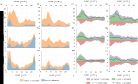
\includegraphics[width=39pc]{error_ECMWF.pdf}
\caption{As in Fig.~\ref{Fig:error_Official}, but for the meridional perturbations.}
\label{Fig:error_ECMWF}
\end{figure*}

Furthermore, it is unclear if the Official forecast's wind fields are intended to be regarded as predictions of the actual winds at a specific location, or a predicted Reynold's average, and if so, at what scale. If we assume the BoM's Official wind forecast intends to represent variability at hourly timescales, and horizontal scales less than 50 kms, then sea-breeze and boundary layer mixing edits appear to have little effect, because the intended reduction in error is washed out by the unpredictable turbulent variability at these scales, and lower errors can be achieved simply by using a coarser resolution unedited model forecast. However, some users may be more interested in whether the variability of the forecast wind field matches those of observations, than in whether the forecast minimises absolute error, and a higher resolution edited forecast will likely perform better than a coarse resolution model in this regard. 

Ambiguity in what the Official forecast represents, and the resulting verification challenge, points to an important role for human forecasters: post-processing and editing model data so that the forecast consistently represents what is of interest to individual users. One barrier to this is that the Official forecast is provided to the national public as a whole, which includes diverse users with different representation needs. Part of the solution may therefore be the development of a secondary economy, either within national weather services like the BoM, or in the private sector, where human forecasters ensure their forecast products consistently represent the ``filtered version of reality" of interest to the end user. This would then help address the representation problem as it applies to the verification of operational forecasts, as the individual user's representation needs could then be taken as the intended representation of the forecast, and appropriate verification metrics chosen accordingly.    

\textcolor{red}{Biases could conceivably be removed by edits, but probably not MSEs?}

Any attempt to validate model data against observations must confront the \textit{representation problem} \citep[e.g.][]{zaron06}. Because models cannot resolve physical processes occurring at sub-grid scales, a value predicted by a model for a given grid-cell must be interpreted as a prediction of the filtered, or Reynolds averaged value over that grid-cell. Therefore, comparing model data with observational data can be an unfair test of model performance, and for this reason model forecasts are often verified against reanalysis hind-casts that use the same model \citep[e.g.][]{lynch14}.

However, the way the representation problem applies to the verification of forecasts issued to the public is more nuanced. In this case, a forecast issued by a national weather service is attempting to represent either reality itself, or the filtered version of reality \textit{that is of interest to the end users.} Thus, \citet{pinson12} disregarded the representation problem entirely, arguing that the end user is not interested in spatiotemporal scales of models, only the ``best forecast" at the time and place of their choice. However, different users will have different ideas about what the ``best" forecast entails. Some users may desire a forecast that minimises absolute error between the forecast and observations, others a forecast that most accurately reproduces the observed wind speed distribution, regardless of temporal details. Ideally, operational forecasts should therefore be assessed according to the specific representation needs of particular end users. 

This presents a challenge for the verification of nationally issued forecasts, as these forecasts are utilised by a variety of end users with diverse representation needs. Moreover, the BoM's forecast is formed from model datasets with different resolutions, and the choice of model guidance can change even over the course of a single day, (e.g.~Fig.~\ref{Fig:case_studies_nt} b). Note the BoM's Official gridded wind forecast exists on a 3 or 6 km, one hour spatiotemporal grid, but is provided to the public through MetEye \citep{bomMetEye19} on a 6 km spatial grid, with wind values given only every 3 hours; hourly data is also available, but is less readily accessible to the public. Furthermore, the BoM verifies its wind forecasts by comparing Official forecast values at each hour UTC, with 10 minute averages of station observations at each hour, with station data typically averaged over the 10 minutes leading up to each hour. These practices suggest that either the Official forecast intends to represent wind fields Reynolds averaged over 6 km, 10 minute spatiotemporal grid cells, or that these averages reflect the representation needs of the typical user. 

Related to the representation problem is the question of how mesoscale models, which run at spatial resolutions of between 1 and 10 km, should be verified. The BoM now regularly runs mesoscale models over some Australian capital cities as part of its daily forecasting routine, and the edits performed by human forecasters are also often mesoscale in nature. Note that mesoscale models resolve topography and its effects on the atmosphere in more detail, and explicitly simulate most convective and boundary layer processes. In this sense they are more realistic than coarser scale models, although they can actually perform worse than coarse models on standard verification scores whenever there are timing or location differences between features in the models and in observations. \citet{mass02} found that in the northwestern United States, mean square errors in forecasts produced using mesoscale models only decreased with resolution down to 10 to 15 km, whereas in the eastern United States where the topography is much flatter, this threshold was considerably larger, at 20 to 40 km. 

\begin{figure*}
\centering
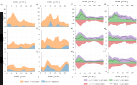
\includegraphics[width=39pc]{error_ACCESS.pdf}
\caption{As in Fig.~\ref{Fig:error_Official}, but for the meridional perturbations.}
\label{Fig:error_ACCESS}
\end{figure*}

\citet{mass02} therefore argued that existing verification approaches needed reform, suggesting that verification could instead be performed on spatially or temporally averaged parameters, an approach now known as \textit{upscaling} \citep{ebert08}. Alternatively, \citet{mass02} argued that ``feature based" identification metrics be developed, which reward models for realistically simulating atmospheric features, even if the timing or location of these features is incorrect. \citet{rife05} developed such a method for the verification of surface winds, defining a wind ``object" as a wind change of at least one standard deviation occurring within a 12 hour interval, then assessing whether a mesoscale model could replicate the ``objects" present in observations.

\begin{table}
\begin{center}
\begin{tabular}{l |c|c}
Airport & Austral Summer & Austral Winter \\
\hline
Darwin  & 6.3 kn& 6.2 kn \\
Brisbane  & 8.6 kn& 7.0 kn \\
Perth  & 11.3 kn& 7.9 kn \\
Sydney  & 12.2 kn & 10.2 kn \\
Adelaide  & 9.5 kn & 10.3 kn \\
Canberra  & 7.4 kn & 7.9 kn \\
Melbourne  & 10.0 kn & 12.1 kn \\
Hobart & 10.0 kn & 8.7 kn
\end{tabular}
\caption{Average 10 m wind speeds for austral winter (June, July August) 2018, and austral summer (December, January, February) 2017/18 across the eight Australian capital city airport weather stations.}
\label{Tab:Speeds}
\end{center}
\end{table}


\bibliographystyle{agsm}
\bibliography{./references.bib}

\end{document}
